\chapter[Referencial Teórico]{Referencial Teórico}

Para inicializar o nosso Referencial teórico de forma concisa em que se alinhe com o que foi proposto com o capítulo 1, é imprescindível abordar o contexto e papel da Fertilização In Vitro, qualidade dos embriões e desafios associados, além de evidenciar como a Inteligência Artificial pode auxiliar a aprimorar as taxas de sucesso de gravidez e minimizar os fatores de risco relacionados a abortos, problemas cromossômicos, além de reduzir os impactos emocionais e físicos associados a esses desafios.

\section{Fertilização In Vitro}

A fertilidade tem sido um tema de grande relevância ao longo da história humana, visto como uma bênção divina em diversas culturas. Civilizações antigas, como a grega e a egípcia, realizavam rituais, usavam amuletos e talismãs, ou buscavam ajuda de divindades para garantir a continuidade de suas linhagens e prosperidade \cite{moura2020}. Esses métodos, embora enraizados em crenças religiosas e espirituais, refletem o desejo universal de superar desafios relacionados à reprodução.

Com os avanços científicos e médicos, a compreensão da fertilidade passou por uma profunda transformação. O primeiro marco documentado foi a inseminação artificial em animais, realizada pelos árabes em 1332 \cite{moura2020}. Essa técnica consiste na introdução do sêmen diretamente no sistema reprodutor da fêmea, otimizando as chances de fertilização \cite{corleta2010}. Em humanos, um dos eventos mais notáveis ocorreu em 1978, com o nascimento de Louise Brown, o primeiro "bebê de proveta" \cite{moura2020}. Este feito foi possível graças ao desenvolvimento da técnica de Fertilização In Vitro (FIV), criada pelo embriologista Robert Edwards e pelo ginecologista Patrick Steptoe. A técnica permitiu a fertilização de óvulos fora do corpo humano e, por sua contribuição revolucionária, Edwards recebeu o Prêmio Nobel de Fisiologia ou Medicina em 2010 \cite{corleta2010}.

As Técnicas de Reprodução Assistida (TRA) compreendem um conjunto de métodos médicos especializados que buscam ajudar indivíduos com dificuldades reprodutivas a alcançarem a concepção \cite{souzamarise2024}. Dentre essas técnicas, a FIV se destaca como a mais avançada e amplamente utilizada \cite{moura2020}. O processo envolve várias etapas, como a estimulação ovariana controlada (uso de medicamentos para estimular a produção de óvulos), coleta de óvulos por punção transvaginal, fertilização em laboratório e posterior transferência dos embriões formados para o útero \cite{moura2020}.

Do ponto de vista técnico, a FIV promove a união do óvulo — gameta feminino — com o espermatozoide — gameta masculino — em ambiente laboratorial \cite{associacaobrasileira2024}. Após a coleta do óvulo (ou ovócito) maduro, ele é fertilizado em laboratório, onde, após a fusão dos gametas, forma-se o embrião. O embrião, que corresponde à fase inicial do desenvolvimento de um organismo, é transferido para o útero, onde, idealmente, se implantará e iniciará a gravidez \cite{associacaobrasileira2024}.

Um avanço significativo no campo da TRA foi a introdução da Injeção Intracitoplasmática de Espermatozoides (ICSI), na década de 1990 \cite{pereira2016}. O ICSI é uma técnica complementar à FIV que consiste na injeção direta de um único espermatozoide no citoplasma do óvulo, utilizando uma micropipeta \cite{pereira2016}. Este método é particularmente útil em casos de infertilidade masculina severa, como baixa contagem de espermatozoides, baixa motilidade ou presença de anomalias estruturais nos espermatozoides \cite{pereira2016}. Embora a FIV possa ser realizada sem o uso de ICSI, este último é frequentemente empregado em casos que exigem maior precisão na fertilização \cite{pereira2016}.

Além de estabelecer as bases da medicina reprodutiva moderna, o nascimento de Louise Brown abriu caminho para avanços na medicina reprodutiva. Desde então, a combinação de avanços médicos e tecnológicos permitiu não apenas a realização da fertilização in vitro, mas também a análise genética detalhada dos embriões \cite{moura2020}. Esses exames identificam anomalias cromossômicas e genéticas, proporcionando uma maior chance de sucesso na implantação e no desenvolvimento de gestações saudáveis.

Os esforços históricos e as inovações científicas ilustram a busca contínua da humanidade por soluções eficazes contra a infertilidade. No próximo tópico, discutiremos detalhadamente a análise de embriões, um procedimento crucial para aumentar as chances de concepção saudável e seu papel na e seu papel na seleção de embriões para a FIV.

\section{Métodos de Avaliação Genética em Reprodução Assistida}

No contexto das Tecnologias de Reprodução Assistida, os métodos de avaliação genética desempenham um papel essencial na identificação de anomalias cromossômicas, como a aneuploidia, que está diretamente relacionada ao número irregular de cromossomos. A qualidade dos embriões é o fator importante para o sucesso da fertilização in vitro \cite{wang2019}, ja que aumenta a chance de uma gravidez bem-sucedida e o nascimento de uma criança saudável, no que diz respeito à ploidia \cite{ramalho2024}. Após décadas de avanços científicos, os testes genéticos tornaram-se cada vez mais precisos, com o desenvolvimento de técnicas sofisticadas e integradas à tecnologia, como a Testagem Genética Pré-implantacional.

Pelo final do século XX, o método do PGT começou a ser usado para realizar o rastreamento de doenças genéticas que possuíam uma alta taxa de incidência nas populações de amostra \cite{yang2024}. Com ele, foi propiciada a triagem de embriões antes da implantação, permitindo a seleção de embriões que possuíam menos riscos \cite{scienceofbiogenetics2024}. Tais métodos incluem a Testagem Genética Pré-implantacional para Doenças Monogênicas (PGT-M), como distrofia miotônica e fibrose cística; para rearranjos estruturais cromossômicos (PGT-SR); para aneuploidias (PGT-A), como Síndrome de Down e Síndrome de Turner; e mais recentemente, o PGT-P para doenças poligênicas \cite{yang2024}. No caso do nosso objeto de estudo, PGT-A, se destaca por sua capacidade de aumentar as chances de implantação embrionária bem-sucedida, reduzir a probabilidade de perdas gestacionais espontâneas e garantir maior probabilidade de nascimento de crianças com o número de cromossomos dos embriões normais\cite{yang2024}. Além disso, o embrião considerado “normal” (euploide) apresenta 23 pares de cromossomos (46 cromossomos no total), sendo metade proveniente do espermatozoide e metade do óvulo. Já o embrião “anormal” (aneuploide) possui uma contagem incorreta de cromossomos, podendo ter cromossomos a mais (trissomias e tetrassomias) ou a menos (monossomias e nulissomias) \cite{cnyfertility2024}. 

O procedimento do PGT-A é dividido em cinco etapas principais, descritas a seguir:

\begin{itemize}
    \item \textbf{Etapa 1: Biópsia de tecido}
    \begin{itemize}
        \item Essa etapa ocorre após os estágios iniciais de fertilização in vitro (FIV), como a estimulação ovariana (uso de medicamentos hormonais para estimular os ovários), coleta de óvulos, fertilização e desenvolvimento embrionário. Quando os embriões atingem a fase de blastocisto (5 a 7 dias após a fertilização), realiza-se uma biópsia para retirar uma pequena amostra de células da camada externa do embrião, chamada trofectoderma. Essa amostra será utilizada para os testes genéticos \cite{cnyfertility2024}.
    \end{itemize}

    \item \textbf{Etapa 2: Envio de amostras e congelamento de embriões}
    \begin{itemize}
        \item As amostras retiradas na biópsia são enviadas para um laboratório de genética especializado. Enquanto isso, os embriões são congelados e armazenados em condições ideais até que o processo de seleção e transferência seja concluído \cite{cnyfertility2024}.
    \end{itemize}

    \item \textbf{Etapa 3: Análise cromossômica PGT-A}
    \begin{itemize}
        \item No laboratório, as amostras passam por uma análise detalhada dos cromossomos para identificar possíveis anomalias. Essa análise é essencial para determinar a viabilidade dos embriões e classificar aqueles com maior chance de resultar em uma gravidez bem-sucedida \cite{cnyfertility2024}.
    \end{itemize}

    \item \textbf{Etapa 4: O Relatório Genético}
    \begin{itemize}
        \item Após a conclusão da análise cromossômica, o laboratório elabora um relatório detalhado indicando o status genético de cada embrião testado, incluindo a contagem cromossômica. Esse relatório é revisado pelo médico especialista, que discute os resultados com os pacientes \cite{cnyfertility2024}.
    \end{itemize}

    \item \textbf{Etapa 5: Seleção de embriões e transferência congelada}
    \begin{itemize}
        \item Com base nos resultados do relatório genético, o médico seleciona os embriões considerados saudáveis (euploides) para a transferência. Os embriões escolhidos são descongelados e preparados para o momento adequado da transferência ao útero \cite{cnyfertility2024}.
    \end{itemize}
\end{itemize}

Os testes genéticos realizados durante a fase de blastocisto são geralmente preferidos por especialistas em reprodução assistida porque essa abordagem envolve a coleta de células do trofectoderma, a camada externa do embrião que futuramente dará origem à placenta, e não diretamente do interior do embrião \cite{leaver2019}. Essa técnica é considerada menos invasiva em comparação com as biópsias realizadas na fase de clivagem, quando o embrião possui apenas algumas células e está em um estágio muito inicial de desenvolvimento \cite{leaver2019}. Na fase de clivagem, a retirada de células do interior do embrião (blastômeros) pode causar danos mais significativos ao embrião, afetando sua capacidade de se desenvolver adequadamente e reduzindo as chances de implantação bem-sucedida no útero \cite{leaver2019}. 

No entanto, é fundamental mencionar que a técnica de micromanipulação necessária para realizar esses procedimentos ainda não foi completamente padronizada. Isso significa que diferentes laboratórios podem adotar práticas distintas para a biópsia embrionária, o que pode resultar em variações na segurança e eficácia dos testes. Além disso, os impactos potenciais dessa intervenção, tanto nos desfechos reprodutivos (como taxas de gravidez e nascimento) quanto na saúde a longo prazo dos bebês nascidos a partir desses embriões, ainda não estão completamente compreendidos.

O PGT-A classifica os embriões em três categorias: euploide (normal, com 46 cromossomos), mosaico (mistura de células normais e anormais) e aneuploide (todas as células com número anormal de cromossomos) \cite{cnyfertility2024}. A Figura~\ref{fig:ResultadosPGT} ilustra os resultados do PGT-A e suas respectivas probabilidades de sucesso gestacional.

\begin{center}
    \begin{figure}[h]
        \captionsetup{font=footnotesize, justification=centering, labelsep=period, position=above}
        \caption{Resultados do PGT-A e suas respectivas probabilidades de sucesso gestacional}
        \label{fig:ResultadosPGT}
        \centering
        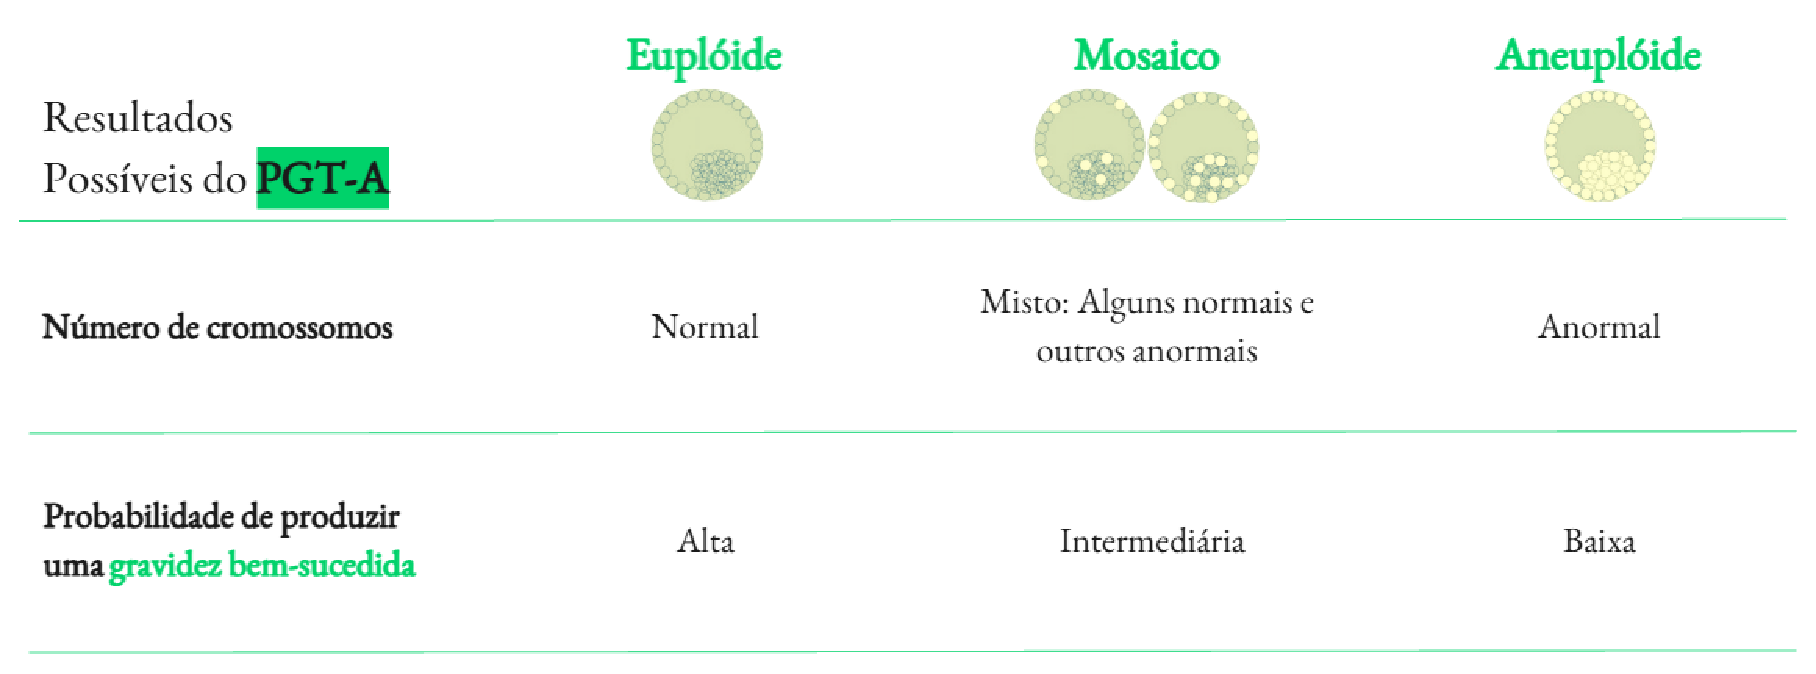
\includegraphics[scale=0.5]{figuras/ResultadosPGT.pdf}
        \vspace{0.3cm} 
        \scriptsize{Fonte: Autoras (2024)}
    \end{figure}
\end{center}
\FloatBarrier

Apesar de suas vantagens, o PGT-A apresenta limitações significativas, como a variabilidade nos resultados das biópsias do trofectoderma e o risco de diagnósticos falso-positivos \cite{gleicher2021}. A The Preimplantation Genetic Diagnosis International Society (PGDIS) e a European Society of Human Reproduction and Embryology (ESHRE) apontam questões críticas, incluindo:

\begin{itemize}
    \item As divergências no conteúdo de DNA aneuploide entre diferentes regiões da trofoectoderma e a massa celular interna demonstram que a biópsia de cinco células pode apresentar resultados variados;
    \item O número exato de células na biópsia nunca é conhecido, o que impossibilita determinar com precisão a porcentagem de DNA aneuploide;
    \item A biópsia da trofoectoderma danifica células individuais, causando vazamento de DNA e contaminação das células vizinhas, dificultando a medição precisa da aneuploidia;
    \item O limiar de 20\% entre euploidia e mosaicismo é baseado apenas na sensibilidade atual do sequenciamento de nova geração (NGS), que não detecta níveis inferiores a 20\% de DNA aneuploide. Consequentemente, qualquer mosaicismo abaixo de 20\% é considerado euploide normal;
    \item Dentro da faixa de mosaicismo (20\% a 80\%), os desfechos de implantação e nascimento são semelhantes, indicando que o uso de limiares rígidos para predizer resultados de FIV é incorreto.
\end{itemize}

Estudos indicam que embriões descartados como aneuploides pelo PGT-A resultaram em nascimentos normais \cite{gleicher2021}, evidenciando a necessidade de revisar as diretrizes para evitar o desperdício de embriões viáveis. A Figura~\ref{fig:biopsiaPGT-A} ilustra a seleção de um pedaço do embrião e como isso pode influenciar a definição da ploidia do mesmo. A biópsia mencionada nas etapas do PGT-A, envolvendo a remoção de uma célula do embrião para análise genética \citeonline{phillips2024}, levantam a preocupação de que a remoção dessas células em crescimento possa comprometer o desenvolvimento do embrião, afetando os resultados neonatais, visto que as técnicas de micromanipulação utilizadas na biópsia não são totalmente isentas de riscos, como observado por \citeonline{leaver2019}.

\begin{figure}[h]
    \captionsetup{font=footnotesize, justification=centering, labelsep=period, position=above}
    \caption{Discrepância potencial entre uma biópsia de células utilizando PGT-A e a composição celular em regiões adjacentes do trofectoderma}
    \label{fig:biopsiaPGT-A}
    \centering
    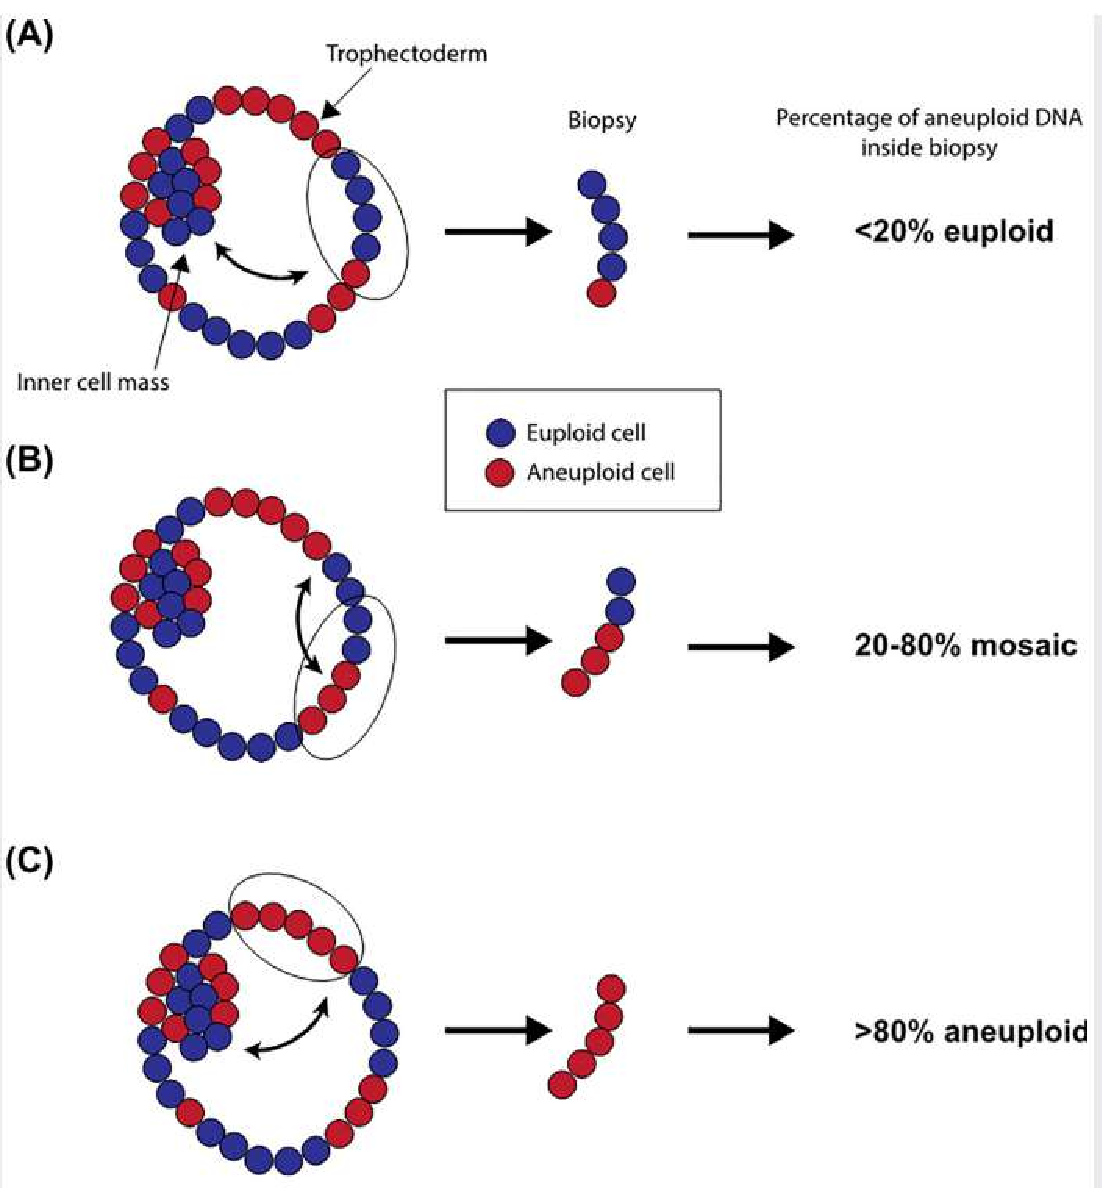
\includegraphics[scale=0.5]{figuras/biopsiaPGT-A.pdf}
    \vspace{0.3cm} 
    \begin{minipage}{\linewidth}
        \centering
        \scriptsize{Fonte: \cite{gleicher2021}}
    \end{minipage}
\end{figure}
\FloatBarrier

Embora o PGT-A permita detectar aneuploidias e aumente as chances de uma gravidez bem-sucedida, ele pode impactar negativamente o potencial de implantação do embrião \cite{gleicher2021}. Por esses motivos, métodos não invasivos estão sendo estudados como alternativas eficientes e seguras, tornando-se cada vez mais relevantes. Um exemplo de técnica não invasiva é a análise morfocinética a partir de imagens obtidas de incubadoras de última geração equipadas com a tecnologia Time-Lapse System.

O TLS é um sistema que captura imagens contínuas dos embriões em desenvolvimento, em intervalos regulares, sem alterar o ambiente de cultivo \cite{moustakli2024}. Essa análise morfocinética, gerada pelas imagens adquiridas pelo TLS, permite o monitoramento quase contínuo do desenvolvimento do embrião, possibilitando a observação de eventos dinâmicos e frequentemente transitórios que não seriam visíveis em observações estáticas \cite{boucret2021}. O uso do TLS não interrompe as condições de cultura, mantendo a viabilidade do embrião durante o processo de monitoramento \cite{moustakli2024}.

As variáveis morfocinéticas incluem aspectos como a forma e a estrutura do embrião (morfológicas) e o movimento e o desenvolvimento do embrião ao longo do tempo (cinéticas), os quais são essenciais para uma análise detalhada de seu progresso \cite{gleicher2021}. Com esse monitoramento contínuo, é possível observar a regularidade das divisões celulares e identificar momentos críticos do crescimento, o que pode auxiliar na diferenciação de embriões euplóides e aneuplóides com base no seu padrão de desenvolvimento \cite{boucret2021}. De acordo com \citeonline{moustakli2024}, o TLS oferece insights valiosos sobre a saúde e o potencial de desenvolvimento dos embriões, utilizando uma abordagem não invasiva, em contraste com a biópsia de embriões. Alguns estudos indicam que, ao ser combinado com pontuações morfocinéticas, o TLS pode aumentar as taxas de implantação e gravidez clínica em comparação aos métodos tradicionais \cite{boucret2021}.

Os dados morfocinéticos coletados pelo TLS oferecem uma nova oportunidade para aprimorar a seleção de embriões em tratamentos de FIV. Considerando uma IA com capacidade para analisar esses dados, seria possível identificar padrões e prever a porcentagem de embriões euplóides. Considerando a aplicação de inteligência artificial (IA) para analisar esses dados, seria possível identificar padrões específicos e prever a probabilidade de embriões serem euplóides, oferecendo uma abordagem mais acessível e financeiramente vantajosa.

\section{Inteligência Artificial}

As dificuldades em definir IA não são, portanto, o resultado de alguma deficiência ou descuido, mas surgem do fato de que fomos incapazes de determinar precisamente qual inteligência desejaríamos replicar artificialmente \cite{sheikh2023}. Dessa forma, definimos a Inteligência Artificial como sistemas que exibem comportamento inteligente ao analisar seu ambiente e tomar ações {–} com algum grau de autonomia {–} para atingir objetivos específicos \cite{sheikh2023}. 

Na medicina reprodutiva, a IA tem se mostrado promissora na melhoria de processos como a fertilização in vitro (FIV). Essa busca por imitar a inteligência humana e entender seus processos cognitivos levou ao desenvolvimento de diversas abordagens, entre elas o Aprendizado de Máquina (Machine Learning, ML), que envolve a capacidade de computadores de interpretar grandes volumes de dados, construir modelos baseados nesses dados e, assim, gerar hipóteses ou previsões sobre o mundo ao seu redor \cite{russell2016}. Na medicina, algoritmos podem ser treinados para reconhecer padrões genéticos em embriões, classificar o melhor embrião para implantação e prever características genéticas de novos embriões. 

Os métodos de ML são geralmente classificados em três tipos principais: aprendizado supervisionado, aprendizado não supervisionado e aprendizado por reforço. Neste estudo, opta-se pelo aprendizado supervisionado como abordagem principal, dada sua eficácia na análise de dados rotulados, permitindo decisões mais precisas e embasadas para otimizar os tratamentos de FIV.

O aprendizado supervisionado consiste no treinamento de algoritmos com base em conjuntos de dados rotulados, nos quais as variáveis de entrada (inputs) e os resultados esperados (outputs) já são conhecidos. O algoritmo aprende a correlacioná-los de forma eficiente \cite{russell2016}, ajustando seus parâmetros com base nas diferenças entre previsões e resultados reais \cite{trask2019}. Uma técnica amplamente usada dentro do aprendizado supervisionado é a classificação, cujo objetivo é atribuir rótulos ou classes pré-definidas aos dados. Por exemplo, no contexto da medicina reprodutiva, um modelo pode ser treinado para diferenciar embriões euploides e aneuploides, aprendendo a reconhecer padrões associados a cada grupo \cite{izbicki2020}.

De maneira geral, um algoritmo de aprendizado supervisionado separa o banco de dados em três subconjuntos: treinamento, validação e teste \cite{izbicki2020}. Na fase de treinamento, o algoritmo identifica padrões nos dados de entrada e os associa às classes desejadas \cite{izbicki2020}. Na validação, um subconjunto de dados não utilizado no treinamento avalia o desempenho do modelo \cite{izbicki2020}, permitindo ajustes nos hiperparâmetros. Após resultados satisfatórios, o conjunto de testes mensura métricas como acurácia, recall e precisão, garantindo o desempenho esperado \cite{izbicki2020}.

A seleção aleatória das amostras para treinamento, validação e teste é uma boa prática \cite{izbicki2020}, evitando problemas decorrentes de ordenações previamente estabelecidas nos bancos de dados. Isso assegura uma visão representativa e imparcial dos dados, fundamental para a construção de modelos robustos e confiáveis \cite{izbicki2020}.

Para a exploração inicial dos dados, utilizaremos o modelo k-Nearest Neighbors (kNN) como ponto de partida, conforme apresentado no livro Aprendizado de Máquina: Uma Abordagem Estatística \citeonline{izbicki2020}. Caso o desempenho e a confiabilidade do kNN não sejam satisfatórios, passaremos a avaliar outros modelos de classificação, como Regressão Linear e Naive Bayes, seguindo esse processo iterativo até encontrarmos um modelo que atenda aos critérios desejados. Se alguns desses modelos demonstrarem resultados satisfatórios, não será necessário explorar os demais.

\subsection{O Algoritmo K-Nearest Neighbor}
O algoritmo K-Nearest Neighbor (KNN) é, em essência, um dos algoritmos mais simples e populares em aprendizado supervisionado, sendo utilizado principalmente em tarefas de classificação e regressão \cite{zhang2016}. Sua principal característica é classificar uma nova observação com base nas classes de seus k vizinhos mais próximos previamente rotulados \cite{zhang2016}. O KNN pode ser considerado um modelo não paramétrico, pois não faz suposições a respeito da distribuição dos dados, o que o torna bastante versátil para uma diversidade de problemas \cite{zhang2016}. É também um algoritmo de aprendizado "preguiçoso" já que não ocorre um processo explícito de aprendizado \cite{zhang2016}.  Então, o algoritmo armazena os dados de treinamento e, na hora de fazer uma predição usa a distância da nova observação para cada exemplo discretamente do conjunto de treinamento para descobrir qual classe ou valor alvo deve usar \cite{zhang2016}.

O desempenho do KNN dé dependente da escolha de k, que são o número de vizinhos que são considerados na classificação \cite{zhang2016}. Valores muito pequenos de k podem a levar a overfitting, já que o modelo se torna sensível ao ruídos contidos nos dados. Valores muito grandes, por sua vez, podem resultar em underfitting pela perda de padrões locais importantes \cite{elkan2011}. Nesse trabalho, utilizaremos num primeiro momento k = 3 e k = 5 para avaliar o desempenho do modelo. Estes valores são adequados uma vez que eles capturam padrão locais sem exagerada sensibilidade ao ruído. Caso necessário, faremos o ajuste no parâmetro k com base nos resultados do conjunto de validação, pois o conjunto de validação é empregado especificamente para otimizar hiperparâmetros.

A métrica de distância adotada foi a distância Euclidiana, uma das mais simples e mais utilizadas. Essa é uma escolha adequada para pequenos conjuntos de dados e de baixa dimensionalidade, como o utilizado neste estudo. Para tais condições a distância euclidiana capta similaridades com eficiência, além de facilitar a interpretação dos resultados \cite{elkan2011}.

O funcionamento do KNN pode ser resumido em três etapas principais de acordo com o \citeonline{elkan2011}:
\begin{itemize}
    \item Armazenar os exemplos de treinamento com suas respectivas etiquetas.
    \item Calcular a distância entre uma nova observação e todos os exemplos armazenados, utilizando uma métrica de similaridade, como a distância Euclidiana.
    \item Selecionar os k vizinhos mais próximos e determinar a classe mais frequente entre eles, atribuindo-a à nova observação.
\end{itemize}

Essa abordagem de classificação por maioria contribui para mitigar o impacto de ruídos ou valores extremos \cite{elkan2011}. Uma prática comum para definir o valor de k é utilizar a raiz quadrada do número total de observações no conjunto de treinamento, embora ajustes específicos sejam feitos dependendo do problema e do conjunto de dados \cite{elkan2011}.

\subsection{Regressão Linear}
A regressão linear é uma técnica estatística utilizada em aprendizado de máquina para expressar relações entre variáveis e para realizar previsões baseadas em dados passados \cite{rodrigues}. É uma abordagem essencial em aprendizado supervisionado, oque visa detectar padrões e criar modelos generalizáveis para dados até então inexistentes \cite{soto}. Segundo \citeonline{santos2007},  é usada para quantificar a associação entre as variáveis, usando frequentemente o coeficiente de correlação de Pearson para avaliar a força e a direção dessa relação. A regressão linear pode ser dividida em dois tipos principais: regressão linear simples e regressão linear múltipla \cite{soto}.

Em um contexto de IA, a regressão linear simples estabelece uma relação matemática entre uma variável dependente \( Y \) e uma única variável independente \( X \), descrita pela equação:
\[
Y = \beta_0 + \beta_1 X + \epsilon,
\]
onde \( \beta_0 \) representa o intercepto, \( \beta_1 \) é o coeficiente angular que expressa a taxa de variação de \( Y \) em relação a \( X \), e \( \epsilon \) é o termo de erro aleatório \cite{rodrigues}. Modelos mais complexos, como a regressão linear múltipla,permitem a inclusão de mais de uma variável independente, aumentando assim a capacidade preditiva e explicativa do modelo \cite{rodrigues}.

A regressão linear é um método paramétrico que requer a suposição de uma relação linear entre as variáveis, o que pode torna-la restritiva quando os padrões não são lineares. Entretanto, técnicas de pré-processamento, como transformações de variáveis e inclusão de termos polinomiais, podem contornar essa limitação e aumentar a capacidade de generalizar do modelo \cite{montgomery2009}.

\subsection{Naive Bayes}
O Naive Bayes é um algoritmo de classificação que se baseia no Teorema de Bayes para estimar a classe mais provável de uma instância, utilizando a probabilidade condicional dos atributos observados \cite{rish2001}. Ele é chamado de "naive" (ou ingênuo) porque parte da suposição de que os atributos são condicionalmente independentes dado a classe. Em outras palavras, presume que a presença ou ausência de um atributo não afeta os outros atributos. Embora essa suposição não seja totalmente realista em muitas situações do mundo real, o algoritmo ainda apresenta resultados impressionantes em diversas aplicações práticas \cite{rish2001}.

De acordo com \citeonline{zhang2004}, o Naive Bayes determina a probabilidade de uma instância pertencer a uma classe específica analisando a distribuição condicional dos atributos. Mesmo com a simplificação imposta pela suposição de independência, o algoritmo muitas vezes alcança resultados comparáveis a métodos mais avançados. O Naive Bayes é particularmente eficaz em problemas de classificação de texto, como análise de sentimentos e classificação de documentos, e em tarefas de diagnóstico médico, como detecção de doenças com base em sintomas ou resultados de exames \cite{rish2001}.


Segundo \citeonline{zhang2004}, A ideia central do Naive Bayes é calcular a probabilidade de uma instância $X = \{x_1, x_2, \dots, x_n\}$ pertencer a uma classe $C_k$ utilizando a fórmula:

$$P(C_k|X) = \frac{P(X|C_k) \cdot P(C_k)}{P(X)}$$

Como o denominador $P(X)$ é constante para todas as classes, o foco do cálculo está em maximizar o numerador, que é proporcional a $P(C_k) \cdot \prod_{i=1}^{n} P(x_i | C_k)$, onde $P(x_i | C_k)$ representa a probabilidade condicional de cada atributo $x_i$, dado a classe $C_k$. O algoritmo calcula essas probabilidades para cada classe e atribui a instância à classe com a maior probabilidade \cite{zhang2004}. 

Em resumo, o Naive Bayes é uma solução simples, rápida e incrivelmente eficaz para muitos problemas de classificação, mesmo quando a suposição de independência não é completamente verdadeira. Essa combinação de praticidade e desempenho o torna uma escolha popular em áreas como processamento de linguagem natural e diagnóstico médico.

\section{Identificação de Padrões Morfocinéticos e Predição de Euploidia com IA e Trabalhos Correlatos}

Os dados que são coletados pela tecnologia do TLS, são chamados de “dados morfocinéticos”, que são definidos como “dados do desenvolvimento dos embriões” \cite{oliveira2024}. Essa informação reunida proporciona noções detalhadas sobre o padrão do desenvolvimento e divisão celular embrionário. Atualmente, após recorrentes estudos sobre esses dados, sabe-se que as “características morfocinéticas dos embriões têm sido associadas à avaliação de sua potência de desenvolvimento”, ou seja, se um embrião analisado pelo TLS tenha um melhor desenvolvimento, ele terá mais probabilidade de ser euplóide, pois um bom desempenho de um embrião é capaz de prever a implantação \cite{yuan2023}.

Os modelos de TLS, de acordo com \citeonline{yuan2023}, tem uma avaliação contínua na etapa do desenvolvimento embrionário por meio de suas imagens e, por observações estáticas, monitora as características do embrião, como tempo e padrões de divisão celular, fornecendo uma base para prever a euploidia. O TLS por si só, não opera com a IA, mas é frequentemente mesclado com essa tecnologia para maiores análises. Um exemplo é o estudo do \citeonline{yuan2023}, o artigo “Development of an artifcial intelligence based model for predicting the euploidy of blastocysts in PGT‐A treatments” o qual teve como objetivo utilizar o TLS e desenvolver um modelo de IA usando uma técnica de regressão logística, para predizer a euploidia de blastocistos—fase do desenvolvimento embrionário que ocorre após a clivagem do óvulo fertilizado—em tratamentos de PGT-A, ajudando a identificar embriões com maiores possibilidades de serem geneticamente normais antes da etapa de transferência. O modelo foi avaliado com uma boa precisão, indicando que ele consegue distinguir entre embriões euploides e aneuploides.

Outro estudo é o de \citeonline{souzarebeca2022}, “Análise da ploidia de embriões humanos por meio da inteligência artificial com o uso de variáveis de morfologia, morfocinética e variáveis relacionadas com a paciente”, também descreve o uso de IA para fazer a predição da ploidia de embriões, classificando os embriões como euplóides e aneuplóides. Para realizar isso, o estudo também combinou dados morfológicas, morfocinéticas e parâmetros clínicos, como o \citeonline{yuan2023}. O modelo utilizado por \citeonline{souzarebeca2022}foi uma rede neural artificial (RNA), treinada justamente para classificar os embriões como citado.

Divergente do trabalho de Zhenya Yuan \cite{yuan2023} e de Rebeca Colauto Milanezi de Souza \cite{souzarebeca2022}, que possuem o objetivo de fazer uma previsão binária de euploidia (mostrando se o embrião em estudo é euploide ou não), o modelo que propomos realizar neste trabalho em questão visa prever a porcentagem de aneuploidia. Com essa diferença de resultado, permitimos uma avaliação mais específica da saúde genética do embrião analisado, ofertando um indicador quantitativo em vez de uma classificação binária.

Para fazer a predição da porcentagem de euploidia, planejamos [citar o modelo de IA que iremos fazer], visando otimizar a precisão da predição, enquanto o modelo dos artigos citados usam uma técnica de regressão logística voltada em previsões binárias.

Com essas diferenças citadas, temos o objetivo de criar uma alternativa menos invasiva e mais acessível para a seleção de embriões na FIV.
